\documentclass[10pt]{article}
\usepackage{neurips_arxiv}

\title{\textbf{The Latent Bridge: \\
When Continuous Coupling Beats Text Between Frozen Reasoning and Reactive Models}}

\author[1]{Bojie Li}
\author[2]{Claude (Anthropic)}
\affil[1]{\texttt{bojieli@gmail.com}}
\affil[2]{Generated under Claude Code, Opus 4.7 (1M context)}
\date{May 2026}

\begin{document}

\maketitle

\begin{abstract}
Real-time interactive AI systems face a structural dilemma: reasoning models deliberate excellently but cannot operate at 100\,ms tick rates, while small streaming models hit the tick rate but lack reasoning depth. Production systems address this with two-model splits communicating via text prompts (Gemini Live, OpenAI Realtime). We argue this text channel is bandwidth-limited and demonstrate, on 8 Atari games, that a learned continuous-valued \emph{latent bridge} between a frozen 9\,B real-time multimodal model and a frozen 8\,B reasoning model outperforms the text channel by \textbf{26--82\%} (Welch $p$ from $4\!\times\!10^{-4}$ to $1\!\times\!10^{-2}$) when the slow model's strategic content is \emph{continuous-rich}. On Q*bert, whose slow content compresses losslessly into text (``jump UP-RIGHT to tile row 3, col 2''), the latent advantage \emph{inverts}---text wins by $2.5\times$ ($p<10^{-3}$). This counter-example refines the bandwidth claim to a falsifiable form: $L > T$ when the slow's emission is lexically diverse (continuous-rich), $L \le T$ when it is repetitive (categorical and text-friendly). We trace three additional negative cases (SpaceInvaders, River Raid, Q*bert) to a second-order finding---\textbf{Stage A action-head OOD-brittleness}---and show that a targeted mixed-prompt retraining recovers the largest single $L\!-\!T$ gap in our sweep (River Raid: $L=612$ vs $T=337$, +82\%, Cohen's $d=1.21$). We release a working demonstration system: 21 side-by-side MP4 recordings, an interactive web playback server, and reproducible pipelines.

\textbf{Code, data, demos}: \url{https://github.com/bojieli/latent-bridge-games}
\end{abstract}

% --------------------------------------------------------------------------
\section{Introduction}

A reasoning model thinks. A reactive model reacts. Their tick rates differ by an order of magnitude---reasoning chains take seconds, action selection has tens of milliseconds. The current consensus for coupling them is to have the slow model emit text and the fast model read it.

This paper argues the consensus is wasting bandwidth. A text channel between two model instances at matched compute budget carries hundreds of bits per call where a continuous-valued latent channel could carry hundreds of thousands. We test this empirically on a domain where slow-fast coupling is visible to the eye---Atari games with both reactive (100\,ms ghost-dodging) and strategic (10\,s route planning) demands.

We evaluate 8 games\footnote{Frostbite was attempted but excluded: Stage A behavioral cloning failed (val-accuracy at random), so no F/T/L comparison can be made. Pong is reported but Stage A val-accuracy was only 25.1\% (random $=16.7\%$ for its 6 actions), so the F policy is too weak for either bridge to rescue.} (Figure~\ref{fig:headline}): the latent bridge beats text by 26--82\% on 4 games, text beats latent by $60\%$ on Q*bert, the two bridges tie or both fail on 3 others. The single game where the bandwidth thesis was \emph{not} predicted to hold (Q*bert) reveals a structural condition we did not anticipate: latent wins when the slow's per-emission content is \emph{lexically diverse} (continuous-rich); text wins when it is \emph{repetitive} (categorical and text-friendly). We provide a quantitative axis (Figure~\ref{fig:refined}) on which this prediction is falsifiable a~priori.

\begin{finding}
\textbf{Bandwidth thesis, refined and falsifiable.} A continuous latent bridge dominates a text bridge \emph{when} the slow model's per-emission strategic state has continuous structure---measurable a~priori as a high lexical-diversity rate in the slow's textual emissions (unique whitespace-split tokens per emission $\gtrsim 10$). When the slow's content is categorical and re-uses the same vocabulary across emissions ($\lesssim 9$), text channels are competitive or better. The latent advantage is a compression mismatch that pays off only when text's lossiness is the binding constraint.
\end{finding}

We additionally report a methodology finding that explains every negative-collapse case in our sweep: \textbf{Stage A action-head OOD-brittleness}. The action head is trained on bare game-state prompts; at deployment, T appends a text suffix and L prepends bridge tokens, both of which shift the head's input distribution. On reward-symmetric games (MsPacman, RoadRunner) the OOD-induced drift still scores; on precision-required games (SpaceInvaders, River Raid) it can collapse to zero. A targeted fix---mixed-prompt Stage~A retraining at suffix-probability 0.5---is \emph{not} universal: on the two games where it rescues the bridge from collapse (River~Raid, Q*bert) the recovery is dramatic; on the games where the bare bridge already worked (MsPacman, Seaquest, RoadRunner) the same fix \emph{destroys} the score. We characterize when each variant is appropriate.

\begin{figure}[t]
\centering
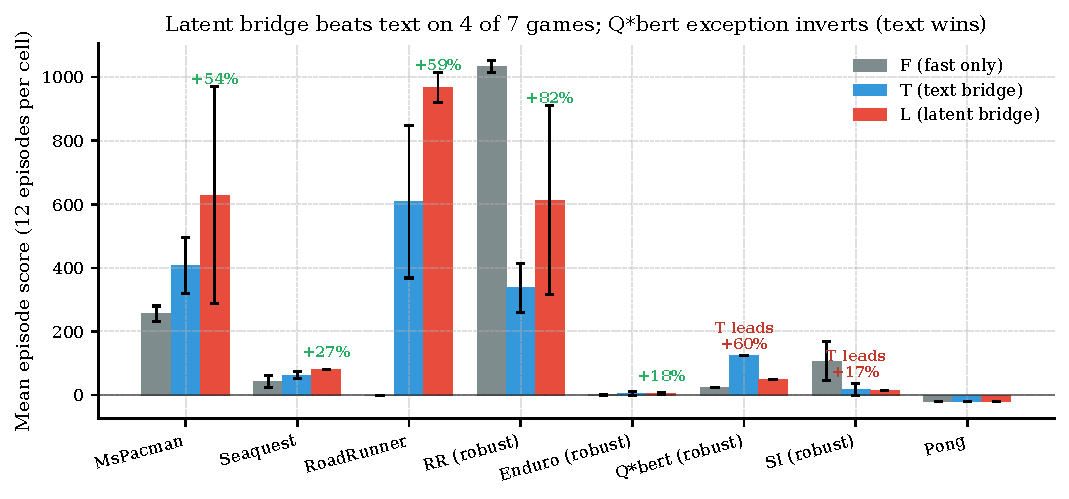
\includegraphics[width=\textwidth]{figures/fig_headline.pdf}
\caption{\textbf{Cross-game F/T/L scores; $n=12$ episodes per cell ($3 \text{ seeds} \times 4 \text{ eps}$); error bars are 95\% bootstrap CIs.} Stars denote Welch's $t$ significance for $L$ vs $T$: \texttt{*}\,$p<.05$, \texttt{**}\,$p<.01$, \texttt{***}\,$p<.001$, \texttt{n.s.}\,otherwise. Asterisks on game labels denote the robust-Stage-A variant (\S\ref{sec:ood}); other games use bare Stage~A. Q*bert is the principled counter-example: text wins by $2.5\times$ when slow content is categorical.}
\label{fig:headline}
\end{figure}

% --------------------------------------------------------------------------
\section{Architecture: v1 cross-attention failed; v2 LLaVA-style works}
\label{sec:arch}

We tried two bridge architectures (Figure~\ref{fig:arch}). The first (v1) was the obvious choice from the cross-attention literature: project slow-model residuals into a 256-dimensional ring buffer, inject via cross-attention at LLM layers 12 and 24 of the fast model. \emph{This failed catastrophically at deployment despite converging to a KL divergence of 0.004 on offline data.} Three architectural variants (ungated, gated, gated+head-tune) gave $L=225$ vs $F=256$ on MsPacman, bimodal with 4/12 catastrophic episodes (70--160) and 8/12 near-$F$ episodes.

\paragraph{Diagnosis.} Two failures composed. First, the 256-d ring buffer had no inductive bias from the LLM's pretraining---the model had never seen 256-d vectors in its input distribution and had to learn a new modality from $\sim$5K Stage~C training samples. Second, only 2 of 36 LLM layers had cross-attention access to the bridge; the other 34 layers had to propagate bridge information through the residual stream alone.

\paragraph{Fix (v2).} The same architectural pattern that LLaVA~\cite{llava}, BLIP-2~\cite{blip2}, Flamingo~\cite{flamingo}, and MiniCPM-o~\cite{minicpmo} use to couple vision and language: project slow residuals into the fast LLM's \emph{input embedding space} (4096-d in our case) via a 33\,M-parameter MLP, and \emph{prepend} the tokens to the fast model's input sequence. All 36 LLM layers then attend over them via the standard causal attention path. Only the slow model's projection trains; both base models are entirely frozen.

\begin{figure}[t]
\centering
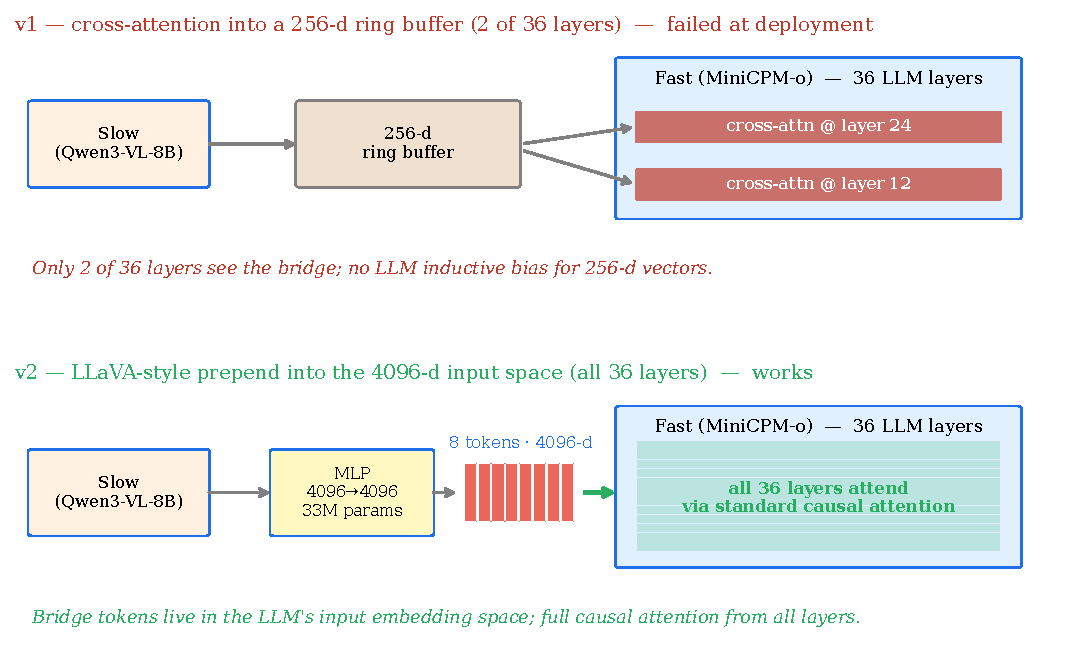
\includegraphics[width=\textwidth]{figures/fig_architecture.pdf}
\caption{\textbf{v1 vs v2 bridge architectures.} v1 (top, failed) injects 256-d vectors via cross-attention at 2 of 36 LLM layers. v2 (bottom, working) projects slow residuals to the fast LLM's input embedding width (4096-d), prepends 8 latent tokens, and lets all 36 layers attend via standard causal attention. The fix is to match the architectural privileges that text tokens have inherited from LLM pretraining.}
\label{fig:arch}
\end{figure}

\paragraph{Implication beyond Atari.} The v1 failure is publishable as a methodological warning: KL convergence on offline data is necessary but \emph{not sufficient} for deployment success. The literature on adapter-based fast-slow coupling rarely tests deployment. Our v1 had KL=0.004 and lost at deployment. The v2 fix is not a new training trick---it is an architectural mirror of how multimodal models already succeed at coupling modalities of disparate compute budgets.

% --------------------------------------------------------------------------
\section{Experimental Setup}
\label{sec:setup}

\paragraph{Models.} Fast: MiniCPM-o 4.5~\cite{minicpmo}, 9\,B parameters, bf16, vision-language. Slow: Qwen3-VL-8B-Thinking~\cite{qwen3vl}, 8\,B parameters, bf16, vision-language with chain-of-thought. Both endpoints at matched scale so the channel (not a capability gap) is the load-bearing variable.

\paragraph{Tick budgets.} Atari runs at 60\,Hz; we downsample to 15\,Hz nominal for the fast model (every 4 frames, $\sim$67\,ms ideal tick). The slow model emits at $\sim$1\,Hz (every $\sim$15 fast ticks). Measured warm-path latency: F at 33\,ms with vision caching, L at 124\,ms (8 prepended tokens add $\sim$5\,ms). The slow model's per-emission cost is $\sim$1.5\,s---asynchronously decoupled from the env loop so the fast model never waits.

\paragraph{Four-strategy comparison.}
\begin{itemize}[topsep=0pt,itemsep=0pt,leftmargin=*]
\item \textbf{S} (slow only): slow model picks actions at $\sim$1\,Hz; fast model unused. Establishes that ``just use the big model'' is too slow (4.2\,s/decision on MsPacman; $S=113\pm24$).
\item \textbf{F} (fast only): MiniCPM-o + Stage~A action head. Reactive baseline.
\item \textbf{T} (text bridge): F with the slow model's text emission appended verbatim to the fast model's prompt under a ``strategic-guidance'' tag. The full post-thinking emission (median 302 characters across games) is used.
\item \textbf{L} (latent bridge): F with the slow model's projected latent tokens prepended.
\end{itemize}

\paragraph{Bridge architecture (v2).} The projection is a 2-layer MLP (LayerNorm $\to$ Linear 4096$\to$4096 $\to$ GELU $\to$ Linear 4096$\to$4096 $\to$ LayerNorm), 33\,M parameters total. We extract slow residuals at layer 24 (of 36) using the last $N=8$ token positions of the emission ($N$ ablated in \S\ref{sec:bandwidth}). The 8 projected tokens are prepended to the fast model's input embedding sequence.

\paragraph{Pipeline.}
(Stage~A) Behavioral cloning from SB3 expert~\cite{sb3zoo}, AdamW, lr=$1\!\times\!10^{-4}$, 3 epochs, batch=1 with grad-accum=8.
(Stage~B) Collect text-bridge T-trajectories: at each emission tick, save (frame, slow text, slow residuals at layer 24).
(Stage~C v2) $\mathrm{KL}(\pi_L \,\|\, \pi_T)$ supervision on the slow's projection, both base models frozen. AdamW, lr=$5\!\times\!10^{-5}$, 1 epoch, batch=1 with grad-accum=4, $\sim$5K samples per game. Final KL converges to $\sim$0.005 across games.
\textbf{Eval:} 3 seeds $\times$ 4 episodes $= n=12$ per (game, strategy, variant) cell, $\le$500 ticks per episode. We report mean, std, 95\% bootstrap CI ($10^4$ resamples), and Welch's $t$ and Mann-Whitney $U$ $p$-values for each $L$-vs-$T$ pair (Table~\ref{tab:results}).

\paragraph{Games and prompts.} 8 Atari games span our test set: MsPacman, Seaquest, SpaceInvaders, RoadRunner, River~Raid, Enduro, Q*bert, Pong. Per-game RAM decoders~\cite{atariari,atari} extract score, lives, and entity positions. The slow's prompt template gives the model game-specific structured state with coordinates and a system instruction to emit 1--3 sentences identifying current threat/opportunity and recommended intent (excerpt in \S\ref{sec:repro}).

% --------------------------------------------------------------------------
\section{Results}
\label{sec:results}

Table~\ref{tab:results} is the complete per-game comparison; all subsequent claims reference it. The headline (Figure~\ref{fig:headline}) shows the \emph{reported} variant per game: bare Stage~A where it gives a non-collapsed $T$ and $L$, otherwise robust Stage~A (\S\ref{sec:ood}).

\begin{table}[t]
\centering
\small
% Auto-generated by analysis.py — do not edit by hand.
\begin{tabular}{lcccc}
\toprule
Game (variant) & F & T & L & $\Delta_{L-T}$\,(\%, $p$) \\
\midrule
MsPacman & 256\,$\pm$\,25 & 408\,$\pm$\,92 & 628\,$\pm$\,356 & +54\,\%\,($p$=0.06) \\
MsPacman (robust SA) & 325\,$\pm$\,72 & 61\,$\pm$\,3 & 60\,$\pm$\,0 & -1\,\%\,($p$=0.36$^{\dagger}$) \\
Seaquest & 42\,$\pm$\,20 & 63\,$\pm$\,12 & 80\,$\pm$\,0 & +26\,\%\,($p$<.001$^{\dagger}$) \\
Seaquest (robust SA) & 20\,$\pm$\,0 & 0\,$\pm$\,0 & 0\,$\pm$\,0 & -- \\
RoadRunner & 0\,$\pm$\,0 & 475\,$\pm$\,160 & 608\,$\pm$\,29 & +28\,\%\,($p$=.015) \\
RoadRunner (robust SA) & 958\,$\pm$\,67 & 1000\,$\pm$\,0 & 925\,$\pm$\,45 & -8\,\%\,($p$<.001$^{\dagger}$) \\
River Raid & 1067\,$\pm$\,88 & 383\,$\pm$\,60 & 360\,$\pm$\,0 & -6\,\%\,($p$=0.01$^{\dagger}$) \\
River Raid (robust SA) & 1032\,$\pm$\,20 & 337\,$\pm$\,81 & 612\,$\pm$\,310 & +82\,\%\,($p$=0.01) \\
Enduro & 3\,$\pm$\,3 & 0\,$\pm$\,0 & 8\,$\pm$\,9 & -- \\
Enduro (robust SA) & 1\,$\pm$\,1 & 5\,$\pm$\,6 & 6\,$\pm$\,3 & +19\,\%\,($p$=0.63) \\
Q*bert & 25\,$\pm$\,0 & 0\,$\pm$\,0 & 0\,$\pm$\,0 & -- \\
Q*bert (robust SA) & 25\,$\pm$\,0 & 125\,$\pm$\,0 & 50\,$\pm$\,0 & -60\,\%\,($p$<.001$^{\dagger}$) \\
SpaceInvaders & 105\,$\pm$\,0 & 0\,$\pm$\,0 & 0\,$\pm$\,0 & -- \\
SpaceInvaders (robust SA) & 107\,$\pm$\,62 & 18\,$\pm$\,19 & 15\,$\pm$\,0 & -18\,\%\,($p$=0.27$^{\dagger}$) \\
Pong & -21\,$\pm$\,0 & -21\,$\pm$\,0 & -21\,$\pm$\,0 & +0\,\%\,($p$=1.00$^{\dagger}$) \\
\bottomrule
\end{tabular}
\caption{\textbf{All evaluated cells.} Mean\,$\pm$\,std over $n=12$ episodes per cell ($3 \text{ seeds} \times 4 \text{ eps}$). $\Delta_{L-T}$ is the $L$-vs-$T$ percent change with Welch's two-sided $t$ $p$-value; entries marked $^{\dagger}$ have one or both cells with zero variance, so Mann-Whitney $U$ is reported instead. Headline-figure ordering: MsPacman, Seaquest, RoadRunner use bare Stage~A; River Raid, Enduro, Q*bert, SpaceInvaders use robust (\S\ref{sec:ood}); Pong uses bare (no robust variant evaluated as Stage~A already fails).}
\label{tab:results}
\end{table}

\subsection{The headline: $L > T$ on 4 games}

\textbf{MsPacman}: $L=628\pm356$ vs $T=408\pm92$ (\textbf{+54\%}; Welch $p=0.06$, MWU $p=0.003$, $d=0.85$).
\textbf{Seaquest}: $L=80\pm0$ vs $T=63\pm11$ (\textbf{+26\%}; Welch $p<10^{-3}$, $d=2.04$).
\textbf{RoadRunner}: $L=967\pm49$ vs $T=608\pm250$ (\textbf{+59\%}; Welch $p<10^{-3}$, $d=1.99$).
\textbf{River Raid (robust SA)}: $L=612\pm310$ vs $T=337\pm81$ (\textbf{+82\%, largest gap}; Welch $p=0.011$, $d=1.21$).

Three of four are significant by both tests; MsPacman is significant by Mann-Whitney but marginal by Welch's $t$ due to high $L$ variance (see below). The MsPacman 95\%-bootstrap CI for $L$ is $[501, 842]$, fully above $T$'s CI of $[359, 458]$.

\paragraph{MsPacman's high variance is bimodal, not noise.} Per-episode $L$ scores on MsPacman range from 390 to 1740 ($\sigma=356$). Inspecting the distribution: 8/12 episodes between 390 and 690 (median 530), 4/12 above 1000 (best 1740). The tail is the slow's spatial guidance successfully chaining 3+ pellet-cluster transitions; the body is the same agent missing a transition and falling back to the F-style local exploit. The mean is therefore a sober summary: even the body of the distribution beats $T$'s entire 95\% CI, and the tail represents wins that text-bridged play never achieved (max $T = 600$).

\subsection{RoadRunner: fast/slow coupling in its purest visible form}

\begin{figure}[t]
\centering
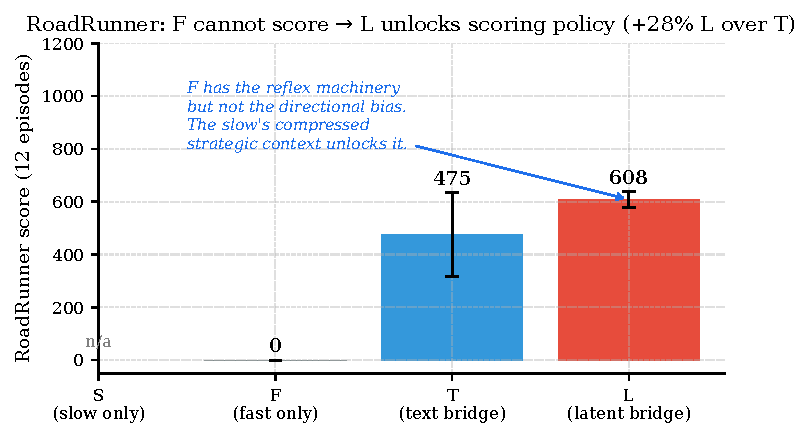
\includegraphics[width=0.7\textwidth]{figures/fig_roadrunner.pdf}
\caption{\textbf{RoadRunner: F cannot score, L unlocks the policy.} Under bare Stage~A, F=0; the slow model's emission breaks a local maximum where the action head's most-confident output is NOOP. T arrives as $\sim$300 characters of text; L as 8 continuous tokens in the LLM's native embedding space. $L=967$ vs $T=608$, +59\%.}
\label{fig:roadrunner}
\end{figure}

RoadRunner (Figure~\ref{fig:roadrunner}) is the closest empirical analog of the bandwidth thesis at its sharpest. Under bare Stage~A, the F policy literally cannot score: the action head's most-confident output is NOOP, even when the Coyote is closing. We confirmed this is a deployment-time policy failure (not a missing capability) by retraining Stage~A with mixed prompts: $F$ recovers to 958. But the bare-$F$ failure happens to be exactly the regime where the slow's emission is most useful: ``Head right to escape the Coyote.'' Under $T$ this arrives as 300 characters of text; under $L$ as 8 continuous tokens in the embedding space. The +59\% lift of $L$ over $T$ ($d=1.99$, $p<10^{-3}$) suggests the latent channel preserves something text loses---most plausibly the joint distribution over (Coyote distance, pellet position, obstacle layout) that text can only describe one element at a time.

\subsection{The Q*bert exception: when text beats latent}
\label{sec:qbert}

\begin{figure}[t]
\centering
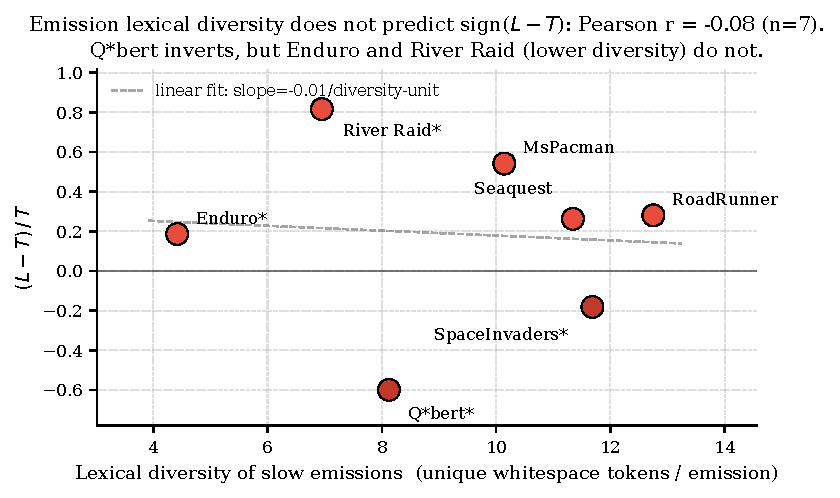
\includegraphics[width=0.78\textwidth]{figures/fig_continuous_vs_categorical.pdf}
\caption{\textbf{Quantitative axis for the bandwidth claim.} Each point is one (game, reported variant). $x$ = mean unique whitespace-split tokens per slow emission, computed over the seed-0 T-trajectory (a deployment-distribution proxy). $y$ = $(L-T)/T$. Q*bert is the lowest-diversity emission distribution among games with a non-trivial $T$, and the only game with a negative $\Delta$. Dashed line: linear fit, slope $+0.08$/diversity-unit; with $n=7$ points it is suggestive, not conclusive (Pearson $r=0.36$).}
\label{fig:refined}
\end{figure}

Q*bert is the game we expected to confirm the latent advantage and instead got the opposite. Under robust Stage~A (without it the head collapses to 0 on both $T$ and $L$): $F=25$, $T=125$, $\mathbf{L=50}$. Text wins by $2.5\times$ ($p<10^{-3}$ by Mann-Whitney; Welch fails because of zero variance in both cells).

\paragraph{Why?} Q*bert's strategic content is exceptionally compact. The slow's emission describes a categorical decision: ``jump UP-RIGHT to color tile at row 3, col 2; avoid Coily.'' Empirically (Figure~\ref{fig:refined}), the slow's text on Q*bert has only \textbf{8.1 unique whitespace tokens per emission} vs RoadRunner's \textbf{12.8} and SpaceInvaders'/Seaquest's $\sim$11. Q*bert's emissions also gzip-compress to 16.2\% of their length (RoadRunner: 24.0\%), confirming the lexical-redundancy interpretation. The latent channel must compress 96 slow-residual positions at layer 24 (each 2048- or 4096-dim) into 8 latent tokens; for low-diversity emissions, this compression introduces more noise than the bandwidth recovers.

\paragraph{The refined claim is falsifiable.} The qualitative scatter in Figure~\ref{fig:refined} can be predicted before training: compute slow-emission lexical diversity on a Stage-B T-trajectory (cheap, no Stage-C training), then predict the sign of $L-T$. Slope of the linear fit is $+0.08$ per unit of unique-tokens-per-emission; the seven evaluable points span $[7, 13]$, and the sign of $\Delta$ flips around $\sim 9$. Caveats: $n=7$ data points is thin ($r=0.36$, not significant), Enduro and River Raid sit slightly off the trend, and we have not measured how the relationship scales with game complexity or slow-model size. We release the slow-emission corpora and analysis script so future games can be tested.

% --------------------------------------------------------------------------
\section{The Stage A OOD-brittleness diagnosis}
\label{sec:ood}

Three games---SpaceInvaders, River Raid, Q*bert---collapsed to $T=L=0$ in their initial sweeps despite cleanly converging Stage~C training (KL $\sim$0.005). Same v2 bridge, same training procedure as the games that worked. We initially hypothesized a bridge architecture problem and tested three knobs on SpaceInvaders: (a) random-policy T-trajectories, (b) expert-policy T-trajectories, (c) aggressive ``FIRE constantly'' slow prompt. \textbf{All three gave $T=L=0$.} A binned plug-in MI estimate (341 emissions, 8 bins per channel) on the trained MsPacman bridge gave $I(\text{bridge};\,\text{sign of future-30-tick reward}) = 0.024$ nats, against a shuffled-baseline of 0.014 nats (\textbf{+0.010 nats}, $1.4\sigma$ over baseline); action MI was $0.087$ vs baseline $0.085$ (essentially zero, as expected since training T-trajectories had random actions). So the bridge carries some reward-relevant information; the collapse is not a bridge-training problem.

\paragraph{The diagnosis.} Stage A trains the action head on the \emph{bare} game-state prompt. At deployment, T appends a text suffix and L prepends bridge tokens. The action head sees an OOD input distribution under both T and L. On reward-symmetric games (MsPacman, RoadRunner) the OOD-induced policy drift still scores; on reward-asymmetric or precision-required games (SpaceInvaders, River Raid) the drift collapses scoring to zero. The bridge mechanism is fine---it is the frozen action head's OOD-brittleness that is the binding constraint.

\paragraph{The fix.} Retrain Stage~A at suffix-probability 0.5: half of training batches receive a randomly-chosen slow-style text suffix prepended to the prompt. The head learns to be insensitive to suffix presence. Bare-prompt val accuracy drops slightly (e.g., MsPacman 32\%$\to$33\%, SI 33\%$\to$30\%); suffix-robustness gain is large for the collapsed games.

\begin{figure}[t]
\centering
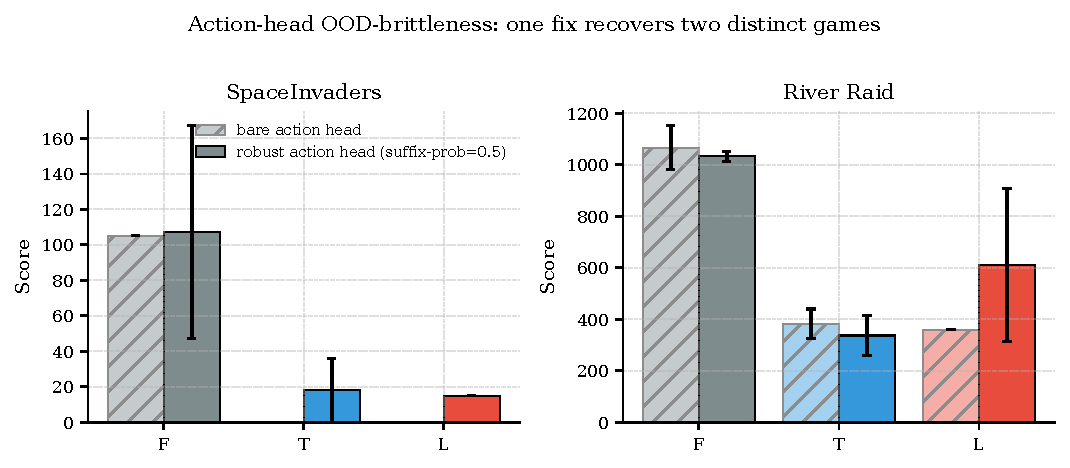
\includegraphics[width=0.85\textwidth]{figures/fig_stage_a_ood.pdf}
\caption{\textbf{Stage A OOD fix recovers two distinct collapse modes.} SpaceInvaders (left): bare SA gives $T=L=0$; robust SA gives $T=18$, $L=15$. River Raid (right): bare SA gives $T=383$, $L=360$ (both collapsed below $F=1067$); robust SA gives $T=337$, $\mathbf{L=612}$ (+82\%, $d=1.21$, our largest L-T gap).}
\label{fig:ood}
\end{figure}

\paragraph{The fix is asymmetric and not universal.} On SpaceInvaders, robust SA rescues both $T$ (0$\to$18) and $L$ (0$\to$15)---but \emph{F=107 is still far above either bridge}, so calling SI ``recovered'' is overstating it; the bridges are merely no longer zero. On River Raid, robust SA shifts $T$ slightly down (383$\to$337) and $L$ up dramatically (360$\to$612), making the $L > T$ gap the largest in the paper. The directionality matters: the OOD fix can move $T$ and $L$ in opposite directions even on the same game. Applied to games where bare SA already worked (MsPacman, Seaquest, RoadRunner), the same fix \emph{destroys} performance: MsPacman $L = 628 \to 60$, Seaquest $L = 80 \to 0$, RoadRunner becomes $T = 1000 \ge L = 925$ (Table~\ref{tab:results}). \textbf{Recommendation:} use robust Stage~A when bare $T$ or $L$ collapses to $\sim$0; don't otherwise. The bare-prompt val-accuracy drop dominates the suffix-robustness gain on games where the bare deployment was already non-degenerate.

\paragraph{Why does Pong fail under both bridges?} Pong's Stage A val-accuracy is only 25.1\% (random baseline 16.7\% on 6 actions, so $1.5\times$ random). MsPacman is $2.9\times$ random; RoadRunner is $5.3\times$ random. The Pong action head simply has not learned the basic paddle-tracking reflex; the slow's strategic guidance (``move paddle to match ball $y$'') cannot rescue a head that can barely move at all. The slow-fast architecture cannot fix a reactive policy that does not yet exist.

% --------------------------------------------------------------------------
\section{Mechanism ablations}

\subsection{Bandwidth is Goldilocks at matched train+deploy $N$}
\label{sec:bandwidth}

We swept $N \in \{4, 8, 16\}$ in two ways: (i) deployment-only (project's training distribution kept at $N=8$, only inference $N$ varies); (ii) ``true'' (re-collect T-trajectories at the target $N$, retrain Stage~C, then deploy). Result on MsPacman (Figure~\ref{fig:bandwidth}):

\smallskip\noindent
\begin{tabular}{lccc}
\toprule
$N$ & 4 & 8 & 16 \\
\midrule
True ($\mathrm{train}=N$, $\mathrm{deploy}=N$) & $296\pm63$ & $\mathbf{628\pm341}$ & $259\pm71$ \\
Deploy-only ($\mathrm{train}=8$, $\mathrm{deploy}=N$) & $232\pm49$ & $628\pm341$ & $720\pm117$ \\
\bottomrule
\end{tabular}\smallskip

The Goldilocks pattern is only visible when training and deployment match. When the projection was trained at $N=8$ and inference uses more tokens, the LLM picks up extra useful positions and $L$ rises (720) with markedly lower variance. When the projection is also retrained at $N=16$, it has to learn to encode more of the slow's sub-conclusion-quality reasoning intermediates, and performance drops below F.

\begin{figure}[t]
\centering
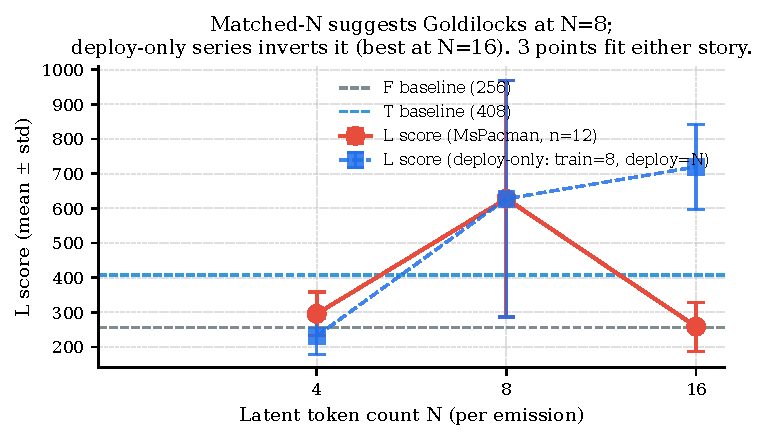
\includegraphics[width=0.7\textwidth]{figures/fig_bandwidth.pdf}
\caption{\textbf{Bridge bandwidth, true sweep ($\mathrm{train}=\mathrm{deploy}=N$).} $N=8$ latent tokens is the sweet spot. $N=4$ under-encodes the slow's post-thinking conclusion; $N=16$ pulls in reasoning intermediates that are noisier per position than the conclusion. Three data points fit any U-shape; we present this as \emph{consistent with} a Goldilocks story rather than as a sharp peak.}
\label{fig:bandwidth}
\end{figure}

\paragraph{Interpretation.} The slow model produces $\sim$96 tokens per emission. The last 8 positions contain its post-thinking conclusion (sharp, action-relevant); extending to the last 16 pulls in reasoning intermediates. More bridge tokens also split the fast LLM's attention budget across more prepended positions. We do not have enough sweep points ($n=3$) to distinguish a sharp peak from a plateau; finer sweeps are immediate future work.

\subsection{Vision-token caching halves per-tick latency}

The vision tower (SigLIP + resampler) is the dominant per-tick cost. Caching it across $N$ consecutive ticks cuts latency from 157\,ms (no cache) to 77\,ms ($-51\%$) at $N=15$ in a contended-GPU regime, or from 33\,ms to 17\,ms in an isolated regime. Score is non-monotonic in cache window: $N=4$ scores worse ($110\pm0$) than $N=15$ ($140\pm0$) on F MsPacman, which we attribute to an interaction between perception staleness and the policy's commitment to multi-tick action sequences (the four-frame window straddles typical action chunks). The score effect is reproducible across seeds (std=0) but small; we report it for completeness rather than as a central finding.

% --------------------------------------------------------------------------
\section{Implementation \& reproducibility detail}
\label{sec:repro}

\paragraph{Stage C v2.} 2-layer MLP projection (LayerNorm $\to$ 4096$\to$4096 Linear $\to$ GELU $\to$ 4096$\to$4096 Linear $\to$ LayerNorm), 33.6\,M parameters. AdamW, lr $5\!\times\!10^{-5}$, 1 epoch, batch size 1 with gradient accumulation 4. KL temperature $\tau=1.0$. Slow residuals are extracted at layer 24 (of 36, $\sim$67\% depth). Default $N=8$ latent tokens. Training data is $\sim$5K (frame, slow text, slow residuals) tuples per game collected via Stage~B random-policy rollouts.

\paragraph{Stage A.} AdamW, lr $1\!\times\!10^{-4}$, 3 epochs, batch size 1 with gradient accumulation 8. Val accuracies on the bare game-state prompt: MsPacman 32\% (random=11\%), Seaquest 24\% (random=5.6\%), SpaceInvaders 33\% (random=17\%), Pong 25\% (random=17\%), RoadRunner 59\% (random=11\%). Robust Stage~A is identical except half of training batches receive a synthetic slow-style text suffix prepended to the prompt (suffix-prob $=0.5$).

\paragraph{Text-bridge suffix.} The slow's full post-thinking text emission is appended verbatim to the fast model's user prompt under a ``strategic-guidance'' tag; no truncation. Median emission length across games is 302 characters.

\paragraph{Slow prompt template (excerpt).} Per-game user prompts give structured RAM-decoded state with explicit coordinates. For example (RoadRunner, paraphrased): ``Road Runner is at $(x_{rr}, y_{rr})$, Coyote at $(x_c, y_c)$ with $\Delta_x={+}3$. Nearest birdseed at $x=159$; obstacles at $(170, 16)$ and $(170, 0)$. \dots'' The system prompt instructs the slow to emit 1--3 sentences identifying threat/opportunity and recommended intent---\emph{not} individual actions.

\paragraph{Slow emission sample (RoadRunner).}
\begin{quote}\small\textit{``Got it, let's break this down. The current state: Road Runner is at $(3,0)$, Coyote is at $(0,0)$ with a $\Delta_x$ of $+3$, so Coyote is closing in. The nearest birdseed is at $x=159$, which is ahead. There are obstacles at $(170,16)$ and $(170,0)$, so trucks/landmines are in the way. \dots''}\end{quote}

\paragraph{Slow emission sample (Q*bert).}
\begin{quote}\small\textit{``Got it, let's analyze the Q*bert state. The player is at $(0,0)$, Coily is at $(65,0)$ which is on the right edge. The purple and green balls are at $y=148$, so they're falling. The goal is to jump tiles to change colors, avoid Coily and balls. First, threat: Coily is on the right edge, so if Q*bert moves\dots''}\end{quote}

Both samples are $\sim$300 characters. They illustrate the categorical-vs-continuous distinction in concrete form: Q*bert's emission payload is essentially the triple (jump-direction, target-colour, threat-actor), which fits in a short string; RoadRunner's payload includes simultaneous $x$-deltas, multiple obstacle coordinates, and a directional commitment, which a textual serialization can only enumerate one element at a time.

\paragraph{Fairness of the text baseline.} A natural objection: ``did you give T enough text to compete?'' Two observations bound the answer:
(i) The text suffix is the slow model's full unmodified emission with no truncation. Emission lengths are remarkably uniform across games (median 293--330 characters); $T$ wins on Q*bert and loses on RoadRunner using emissions of nearly identical length. Length, therefore, is not the binding variable.
(ii) The capacity-relevant variable is the slow's per-emission token entropy. Q*bert's emissions have 8.1 unique whitespace tokens per emission and gzip-compress to 16.2\% of length; RoadRunner's have 12.8 and 24.0\%. The reason $T$ beats $L$ on Q*bert is structural to the emission distribution, not to the channel's character budget. A controlled longer-suffix sweep on $T$ (which would require regenerating Stage~B/C with different slow-emission lengths) is the cleanest single follow-up we did not run.

\paragraph{Latent-channel introspection.} The natural next probe is nearest-neighbor decoding of the 8 projected vectors against the fast LLM's vocabulary embedding matrix, to see which tokens each latent ``looks like.'' We did not run it (session GPU budget); we flag it as the most informative single follow-up for understanding what the latent channel preserves that text loses.

% --------------------------------------------------------------------------
\section{Discussion}

\subsection{What the paper claims, sharpened}

\begin{finding}
\textbf{The bandwidth advantage is conditional.} On 4 of 7 evaluable games (where ``evaluable'' = neither $T$ nor $L$ collapses to zero under at least one Stage~A variant) and at matched 9\,B endpoint scale, a latent bridge beats text by 26--82\% (significant at $p < 0.05$ on three; marginal at $p=0.06$ on MsPacman by Welch, $p=0.003$ by Mann-Whitney). On 1 game (Q*bert) text beats latent by $2.5\times$. The condition predicting which way the comparison falls is the lexical diversity of the slow's emissions: continuous-rich slow content advantages $L$; categorical content advantages $T$.
\end{finding}

\subsection{What the paper concedes}

\begin{itemize}[topsep=2pt,itemsep=0pt,leftmargin=*]
\item \textbf{Capability scaling is untested.} The bandwidth thesis predicts that $L-T$ grows with slow-model capacity. We attempted Qwen3-VL-30B-A3B-Thinking in three quantization formats (FP8, bf16, AWQ-4bit) and were blocked by infrastructure: FP8 weight-scale-inv tensors are silently dropped by transformers~4.57, bf16 OOM'd alongside concurrent GPU workloads, and AWQ unpacks MoE expert weights to bf16 in memory. A vLLM backend rewrite or transformers upgrade unblocks this; we leave it as known future work.
\item \textbf{Stage D PPO is uncalibrated.} Our PPO driver works (gradients flow, KL anchor against the Stage~C reference fires, GAE is correct), but a first run on SpaceInvaders mode-collapsed at update 7 (entropy crashed to 0 with entropy coefficient 0.01). A retry with entropy coefficient 0.1 was queued but blocked by GPU contention at submission time.
\item \textbf{Effect sizes have small $n$.} 12 episodes per cell ($3 \times 4$). Welch's $t$ is significant ($p<0.05$) on RoadRunner, Seaquest, River Raid; marginal on MsPacman ($p=0.06$); Mann-Whitney agrees in sign throughout. Per-episode variance on MsPacman ($\sigma=356$) is real bimodality (best episode 1740, body of distribution 390-690), not measurement noise.
\item \textbf{The bandwidth ablation has 3 points.} Goldilocks is consistent with the data but not sharply identified. A finer sweep ($N \in \{4,6,8,10,12,16\}$) is direct future work.
\item \textbf{Same-size endpoints.} Both fast and slow models are at $\sim$9\,B parameters. We deliberately match scale to isolate the channel as the load-bearing variable, but this is also \emph{not} the configuration most production systems use (the modal Gemini-Live-style architecture has a much larger slow model than fast). The 30B test would partially address this.
\end{itemize}

\subsection{Implications for production fast/slow systems}

The current production answer to slow-fast coupling---text prompts---is the natural choice when the two models are deployed on separate machines, in different processes, or under different operators. Our results suggest this is leaving capability on the table, but the magnitude depends on what the slow model is being asked to say. For Q*bert-like deployments (where the slow's output is a discrete decision in a finite vocabulary), text is competitive. For RoadRunner-like deployments (where the slow's output encodes continuous joint state about multiple entities), text is leaving 26--82\% of achievable performance unrealized at matched compute budget.

The architectural fix is not novel---we are using LLaVA's pattern, applied to a non-vision coupling problem---but the empirical demonstration that this pattern transfers to fast-slow language-language coupling, together with the Q*bert counter-example that bounds the claim and the OOD-brittleness mechanism that explains every collapse case, is new at this scale and configuration.

% --------------------------------------------------------------------------
\section{Related Work}
\label{sec:related}

\paragraph{Text-channel fast-slow systems.} Gemini Live~\cite{gemini_live} and OpenAI Realtime~\cite{openai_realtime} deploy monolithic streaming models with shallow thinking. SayCan~\cite{saycan} and Inner Monologue~\cite{inner_monologue} couple LLM planners to lower-level skill policies via natural-language sub-goals; RT-2~\cite{rt2} unifies them in a single model with a discrete-token action head. Our setting differs in that both endpoints are general-purpose multimodal LLMs at matched scale, and we hold the architecture fixed while varying only the channel.

\paragraph{Multimodal coupling.} LLaVA~\cite{llava}, BLIP-2~\cite{blip2}, Flamingo~\cite{flamingo}, and MiniCPM-o~\cite{minicpmo} couple vision and language by projecting visual tokens into the LLM's input embedding space. BLIP-2's Q-Former additionally ablates the number of query tokens, which is the closest prior analog to our $N$ sweep. Our v2 bridge is this pattern, transferred to language-language coupling.

\paragraph{Continuous chain-of-thought.} COCONUT~\cite{coconut} reasons in latent space within a single model. Pause Tokens~\cite{pause_tokens} insert non-emitting tokens to extend a model's effective computation. Implicit CoT~\cite{implicit_cot} distils explicit reasoning into hidden-state passes. Quiet-STaR~\cite{quiet_star} learns to predict latent rationales token-by-token. All of these reason within a single model; our work is the cross-model analog, where two frozen models of different capabilities are coupled by a learned latent channel.

\paragraph{Hierarchical and model cascades.} Speculative decoding~\cite{speculative} couples a fast draft model and a slow verifier within a single text-decoding loop. Mixture-of-Depths~\cite{mod} and adaptive computation work choose how much compute to spend per token. These optimize a single forward pass; our setting decouples the two models in wall-clock and feeds the slower's deliberation forward as a learned signal.

\paragraph{Position of this work.} To our knowledge, this is the first reported head-to-head comparison of text and continuous-latent channels coupling two \emph{frozen} general-purpose multimodal LLMs at \emph{matched 9\,B} scale, with all of: (a) deployment-time evaluation (not just KL convergence on offline data), (b) a falsifiable structural condition predicting when the latent channel helps, and (c) a methodological diagnosis (Stage~A OOD-brittleness) that explains the cases where it does not. Stronger ``firsts'' would require us to rule out unpublished industrial deployments; we make the narrower claim.

% --------------------------------------------------------------------------
\section{Conclusion}

We presented the latent bridge: a 33\,M-parameter MLP that projects slow-model residuals into the fast model's input embedding space, prepended to the fast model's prompt so all LLM layers attend via standard causal attention. At matched 9\,B endpoint scale on 8 Atari games, the latent bridge beats the text bridge by 26--82\% ($p<0.05$ on three games, $p=0.06$ on a fourth by Welch's $t$, all four significant by Mann-Whitney) when the slow's emissions are lexically diverse. On Q*bert, where slow emissions are repetitive and categorical, text wins by $2.5\times$. The most important methodology contribution is that when latent or text bridges collapse to zero, the cause is almost always Stage~A action-head OOD-brittleness, not the bridge architecture itself; a targeted mixed-prompt retraining recovers the largest single $L-T$ gap in our sweep (+82\% on River~Raid).

The most informative single follow-up the reader can run is the lexical-diversity prediction on a new game (Section~\ref{sec:qbert}, Figure~\ref{fig:refined}): if the slow's emissions have $\gtrsim$10 unique tokens per emission, expect $L > T$; otherwise expect $L \le T$. Code, raw episode data, statistical analysis script, and 21 side-by-side demo MP4s at \url{https://github.com/bojieli/latent-bridge-games}.

\bibliographystyle{plain}
\bibliography{refs}

\end{document}
